\chapter{定积分}
\thispagestyle{empty}
\noindent
\begin{minipage}{0.55\linewidth}
	\section{定积分的基本概念}
	\subsection{曲边梯形的面积}
\hspace*{2em} 设$y=f(x)$在区间$[a,b]$上连续非负。由直线$x=a$,$x=b$,$y=0$及曲线$y=f(x)$所围成的图形称为\highlight{dy}{\index{QBTX@曲边梯形}曲边梯形},其中曲线弧称为\highlight{dy}{曲边},如图 \ref{曲边梯形} 所示。

\hspace*{2em} 下面用\highlight{dy}{\index{YSF@元素法}元素法}详细地说明曲边梯形面积的求法。\\
\hspace*{2em} (1)\enspace\textbf{分割}。用任意一组分点把区间$[a,b]$分成长度为$\Delta x_i$($i=1,2,\cdots,n$)的$n$的小区间$[x_{i-1},x_i]$,相应地把曲边梯形分成$n$个窄曲边梯形,第$i$个窄曲边梯形的面积设为$\Delta S_i$,则
\end{minipage}
\begin{minipage}{0.45\linewidth}
	\centering
	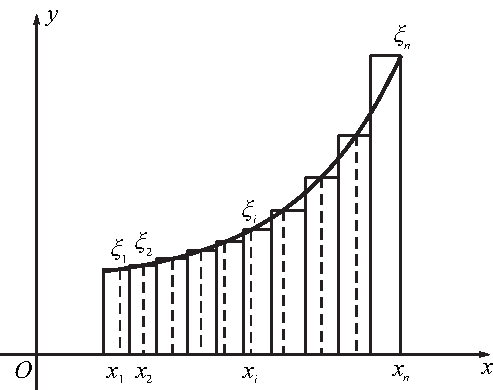
\includegraphics[width = 0.95\linewidth]{pic/C-4/曲边梯形}
	\vspace*{-1em}
	\captionof{figure}{曲边梯形的面积}
	\label{曲边梯形}
\end{minipage}

\begin{equation}
	S=\sum_{i=1}^{n}\Delta S_i
\end{equation}
\hspace*{2em} (2)\textbf{计算$\Delta S_i$的近似值}(利用窄曲边梯形的面积$\approx$窄边矩形的面积=高$\times$宽,在每个小区间$[x_{i-1},x_i]$上用其中某一点$\xi_i$处的高来近似代替同一个小区间上窄矩形的变高)
\begin{equation}
	\Delta S_i\approx f(\xi_i)\Delta x_i(x_{i-1}\leq \xi_i\leq x_i)
\end{equation}
\hspace*{2em} (3)\textbf{求和},得$S$的近似值
\begin{equation}
	S=\sum_{i=1}^{n}\Delta S_i\approx\sum_{i=1}^{n} f(\xi_i)\Delta x_i
\end{equation}
\hspace*{2em} (4)\textbf{求极限},记$\lambda=\text{max}\{\Delta x_i,1\leq i\leq n\}$,($\lambda$的几何意义是所有分得的小区间中长度最大的区间。当$\lambda\to0$时,所有的小区间长度都趋于0,这个时候分得的每个区间足够小,上式便不是估计式,而是等式)得
\begin{equation}
	S=\sum_{i=1}^{n}\Delta S_i=\lim\limits_{\lambda\to 0}\sum_{i=1}^{n}f(\xi_i)\Delta x_i
\end{equation}
\subsection{定积分的定义}
通过计算曲边梯形的面积,我们可以类比得到定积分的定义。
\\ 

\vspace*{-1em}
\defination[定积分定义]
设函数$f(x)$在$[a,b]$上有界,在区间$[a,b]$中任意插入若干个分点
\begin{equation}
	\nonumber
	a=x_0<x_1<x_2<\cdots<x_{n-1}<x_n=b
\end{equation}
把区间$[a,b]$分成$n$个小区间:
\begin{equation}
	[x_1,x_2],[x_2,x_3],\cdots,[x_{n-1},x_n]
\end{equation}
各个小区间的长度依次为:
\begin{equation}
	\nonumber
	\Delta x_1=x_2-x_1,\Delta x_2-x_3,\cdots,\Delta x_n=x_n-x_{n-1}
\end{equation}
在每个小区间$[x_{i-1},x_i]$上任取一点$\xi_i(x_{i-1}\leq \xi_i\leq x_i)$,作函数值$f(\xi_i)$与小区间长度$\Delta x_i$的乘积$f(\xi_i)\Delta x_i$,并求和
\begin{equation}
	S=\sum_{i=1}^{n}f(\xi_i)\Delta x_i
\end{equation}
\hspace*{2em} 记$\lambda=\text{max}\{\Delta x_i,1\leq i\leq n\}$\footnote{无特殊说明,在本章节中$\lambda$都表示$\max \{\Delta x_i,1\leq x_i\leq n\}$},如果$\lambda\to 0$时,上式的极限总存在,且与闭区间$[a,b]$的分法及点$\xi_i$的取法无关,那么称这个极限为函数$f(x)$在区间$[a,b]$上的\highlight{dy}{\index{DJF@定积分}定积分}(简称\highlight{dy}{\index{JF@积分}积分}),记作
\begin{equation}
	\int_{a}^{b}f(x)\,\d x=\lim\limits_{\lambda\to0}\sum_{i=1}^{n}f(\xi_i)\Delta x_i
\end{equation}
\hspace*{2em} 其中函数$f(x)$叫做\highlight{dy}{\index{BJHS@被积函数}被积函数},$f(x)\d x$叫做\highlight{dy}{\index{BJBDS@被积表达式}被积表达式},$x$叫做\highlight{dy}{\index{JFBL@积分变量}积分变量},$a$叫做\highlight{dy}{\index{JFXX@积分下限}积分下限},$b$叫做\highlight{dy}{\index{JFSX@积分上限}积分上限},$[a,b]$叫做\highlight{dy}{\index{JFQJ@积分区间}积分区间}。\\
\hspace*{2em} 由于积分的定义与极限有关,故我们也可以用$\varepsilon-\delta$语言来表述定积分的定义。
\\ \hspace*{2em} 设有常数$I$,如果对于任意给定的正数$\varepsilon$,总存在一个正数$\delta$,使得对于区间$[a,b]$的任何分法,不论$\xi_i$在$[x_{i-1},x_i]$中怎样选取,只要$\lambda=\max\{\Delta x_i,1\leq i\leq n\}<\delta$,总有
\begin{equation}
	\bigg|\sum_{i=1}^{n}f(\xi_i)\Delta x_i-I \,\bigg|<\varepsilon\vspace*{-1em}
\end{equation}
\noindent 成立,那么我们称$I$函数$f(x)$在区间$[a,b]$上的定积分,记作$\di\int_{a}^{b}f(x)\,\d x$.
\warn[\hspace*{2em} 定积分的值只与被积函数和被积区间有关,而与积分变量的记法无关。例如
\begin{equation}
	\int_{a}^{b}f(x) \,\d x=\int_{a}^{b}f(t) \,\d t=\int_{a}^{b}f(u) \,\d u\vspace*{-1em}
	\end{equation}
\hspace*{2em} $\di\sum_{i=1}^{n}f(\xi_i)\Delta x_i$通常称为$f(x)$的积分和。如果$f(x)$在{$[a,b]$}上的定积分存在,那么就称$f(x)$在{$[a,b]$}上可积。]
\noindent \textbf{【补充\hspace{1em} 积分存在的条件】}\\

\vspace*{-1em}
\theorem[积分存在条件1]
设函数$f(x)$在$[a,b]$上连续,则$f(x)$在$[a,b]$上可积。\\

\vspace*{-1em}
\theorem[积分存在条件2]
设函数$f(x)$在$[a,b]$上有界,且只有\textbf{有限个}间断点,则$f(x)$在$[a,b]$上可积。
下面只给出一个不可积的函数:狄利克雷函数(Dirichlet)函数
\begin{equation}
	\nonumber
	D(x)=\left\{
		\begin{aligned}
			& \,1,x\in Q\\
			& \,0,x\in q&
		\end{aligned}
		\right.
\end{equation}
这个函数有无穷个间断点,故它是不可积的函数。

\noindent
\begin{minipage}{0.6\linewidth}
	\subsection{定积分的几何意义}
\hspace*{2em} 如图 \ref{定积分的几何意义} 所示,定积分$\di\int_{a}^{b}f(x) \,\d x$表示曲线$y=f(x)$,两条直线$x=a,x=b$与$x$轴上方所围成的曲边梯形减去$x$轴下方所围成的图形面积。例如$\di\int_{a}^{b}f(x) \,\d x=S_2-S_1-S_3$.
\vspace*{1.5em}

\section{定积分的运算法则}
\subsection{定上下限定积分的性质}
\hspace*{2em} 首先,我们对定积分的定义再补充两个规定:
\end{minipage}
\begin{minipage}{0.4\linewidth}
	\centering
	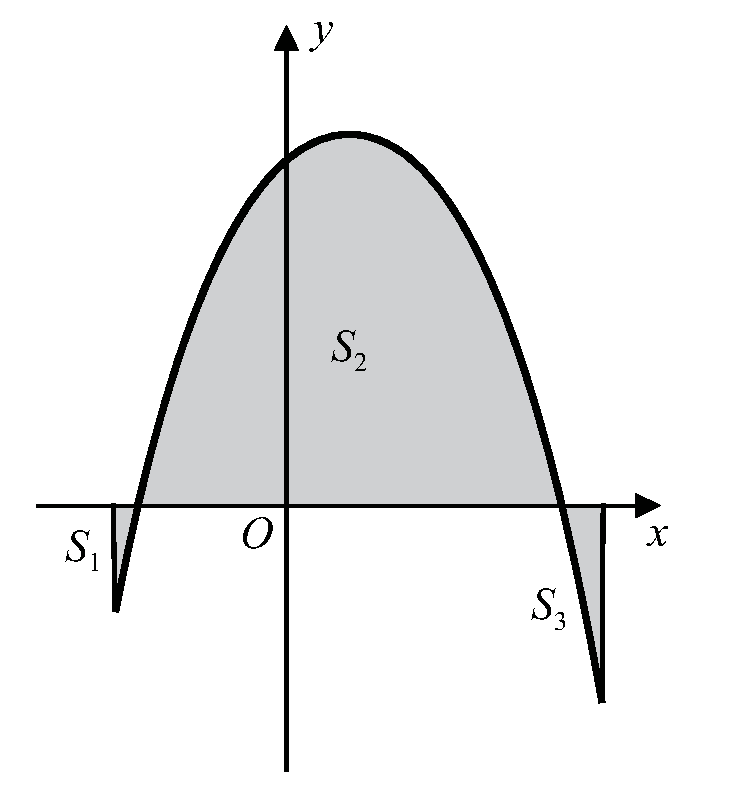
\includegraphics[width=0.75\linewidth]{pic/C-4/定积分几何意义}
	\vspace*{-1em}
	\captionof{figure}{定积分的几何意义}
	\label{定积分的几何意义}
\end{minipage}

\begin{equation}
	\int_{a}^{b}f(x) \,\d x=0
\end{equation}
\begin{equation}
	\int_{a}^{b}f(x) \,\d x=-\int_{b}^{a}f(x) \,\d x
\end{equation}
由上式可知,交换定积分的上下限时,定积分的绝对值不变而符号相反。\\

\vspace*{-1em}
\theorem[定上下限积分性质1]
设$\alpha$与$\beta$均为常数,则
\begin{equation}
	\int_{a}^{b}[\alpha f(x)+\beta g(x)] \,\d x=\alpha\int_{a}^{b}f(x) \,\d x+\beta\int_{a}^{b}g(x) \,\d x
\end{equation}
\proof $\di\int_{a}^{b}[\alpha f(x)+\beta g(x)] \,\d x=\lim\limits_{\lambda\to0}\sum_{i=1}^{n}[\alpha f(\xi_i)+\beta g(\xi_i)]\Delta x_i$\vspace{-1em}\\
\hspace*{14.7em}$=\di\lim\limits_{\lambda\to0}\sum_{i=1}^{n}\alpha f(\xi_i)\Delta x_i+\lim\limits_{\lambda\to0}\sum_{i=1}^{n}\beta g(\xi_i)\Delta x_i$\\
\hspace*{14.7em}$=\di\alpha\lim\limits_{\lambda\to0}\sum_{i=1}^{n}f(\xi_i)\Delta x_i+\beta\lim\limits_{\lambda\to0}\sum_{i=1}^{n}g(\xi_i)\Delta x_i$\\
\hspace*{14.7em}$=\alpha \di\int_{a}^{b}f(x)\,\d x+\beta \int_{a}^{b}g(x)\,\d x$\\

\theorem[定上下限积分性质2]
设$a<c<b$,则
\begin{equation}
	\int_{a}^{b}f(x) \,\d x=\int_{a}^{c}f(x) \,\d x+\int_{c}^{b}f(x) \,\d x
\end{equation}
\proof 因为函数$f(x)$在区间$[a,b]$上可积,所以不论把区间$[a,b]$怎样分,积分和的极限都不会改变,因\vspace{-0.5em}\\ 此,\textbf{在分区时,可以使$c$点永远是个分点}。那么,$[a,b]$上的积分和等于$[a,c]$上的积分和加上$[c,b]$上的积分和,即
\begin{equation}
	\sum_{[a,b]}f(\xi_i)\Delta x_i=\sum_{[a,c]}f(\xi_i)\Delta x_i+\sum_{[c,b]}f(\xi_i)\Delta x_i
\end{equation}
令$\lambda\to0$,两端同时取极限,即得
\begin{equation}
	\int_{a}^{b}f(x) \,\d x=\int_{a}^{c}f(x) \,\d x+\int_{c}^{b}f(x) \,\d x
\end{equation}
\hspace*{2em} 实际上,由于有了定积分的补充定义,无论$a,b,c$的位置如何,上式都成立。\\
\hspace*{2em} 这个性质表明定积分对于积分区间具有\textbf{可加性}。\\

\theorem[定上下限积分性质3]
\label{theorem:1}
如果在区间$[a.b]$上$f(x)>0$,那么
\begin{equation}
	\int_{a}^{b}f(x) \,\d x\geq0
\end{equation}
\proof 因为$f(x)\geq 0$,所以$f(\xi_i)\geq0$,又由于$\Delta x_i(i=1,2,\cdots,n\geq0)$,所以\vspace*{-1em}
\begin{equation}
	\sum_{i=0}^{n}f(\xi_i)\Delta x_i\geq0 \Rightarrow \int_{a}^{b}f(x) \,\d x=\lim\limits_{\lambda\to0}\sum_{i=1}^{n}f(\xi_i)\Delta x_i\geq 0
\end{equation}

\theorem[定上下限积分性质4]
\label{theorem:2}
如果在区间$[a,b]$上$f(x)\geq g(x)$,那么
\begin{equation}
	\int_{a}^{b}f(x) \,\d x\geq \int_{a}^{b}g(x) \,\d x
\end{equation}
\proof 因为$f(x)-g(x)\geq0$,由\ref{theorem:1}\hspace*{0.3em}得
\begin{equation}
	\int_{a}^{b}f(x)-g(x) \,\d x=\int_{a}^{b}f(x) \,\d x-\int_{a}^{b}g(x) \,
	\d x\geq0
\end{equation}
证毕。\\

\vspace*{-1em}
\theorem[定上下限积分性质5]
\label{theorem:3}
设$M$及$m$分别是函数$f(x)$在区间$[a,b]$上的最大值及最小值,则
\begin{equation}
	m(b-a)\leq \int_{a}^{b}f(x) \,\d x\leq M(b-a)
\end{equation}
\proof 因为$m\leq f(x)\leq M$,由 \ref{theorem:2}\hspace*{0.3em}得
\vspace*{-1em} 
\begin{equation}
	\nonumber
	m(b-a)=\int_{a}^{b}m \,\d x\leq \int_{a}^{b}f(x) \,\d x\leq \int_{a}^{b}M \,\d x=M(b-a)
\end{equation}
证毕。\\
\hspace*{2em} 这个定理为我们\textbf{估计定积分的值}提供了一种简单的方法,例如:
\begin{equation}
	\nonumber
	1=(2-1)\times1^3\leq \int_{1}^{2}x^3 \,\d x\leq (2-1)\times2^3=8
\end{equation}

\vspace*{-1em}
\theorem[积分中值定理]
\label{theorem:4}
如果函数$f(x)$在积分区间$[a,b]$上连续,那么在区间$[a,b]$上至少存在一个点$\xi$,使得
\begin{equation}
	\int_{a}^{b}f(x)\,\d x=f(\xi)(b-a)(a\leq\xi\leq b)
\end{equation}
\proof 设$M$及$m$分别是函数$f(x)$在区间$[a,b]$上的最大值及最小值,则由\ref{theorem:3}\hspace*{0.3em} 得
\begin{equation}
	\nonumber
	m\leq\frac{1}{b-a}\int_{a}^{b}f(x) \,\d x\leq M
\end{equation}
又$m\leq f(x)\leq M$,由介值定理可知在区间$[a,b]$上至少存在一个点$\xi$,使得$f(\xi)=C\in[m,M]$.\vspace{0.5em}\\
而由于定积分$\di\frac{1}{b-a}\int_{a}^{b}f(x)\,\d x$也是一个具体的常数,且$\di m\leq\frac{1}{b-a}\int_{a}^{b}f(x) \,\d x\leq M$,\\
由于$C\in [m,M]$是任意的数,则我们取$C=\di\frac{1}{b-a}\int_{a}^{b}f(x) \,\d x$,那么\\
在区间$[a.b]$上至少存在一个点$\xi$,使得
\begin{equation}
	\nonumber
	f(\xi)=\frac{1}{b-a}\int_{a}^{b}f(x)\,\d x \Rightarrow \int_{a}^{b}f(x)\,\d x=f(\xi)(b-a).
\end{equation}

\noindent
\begin{minipage}{0.5\linewidth}
	\hspace*{2em} 积分中值公式也有几何解释如下:\\
\hspace*{2em} 如图 \ref{积分中值定理几何意义} 所示,在区间$[a,b]$上至少存在一个点$\xi$使得以区间$[a,b]$为底边的,以曲线$y=f(x)$为曲边的曲边梯形的面积等于同一底边而高为$f(\xi)$的一个矩形的面积。\\ 
\hspace*{2em} 按积分中值公式可得:
\begin{equation}
	\nonumber
f(\xi)=\frac{1}{b-a}\int_{a}^{b}f(x) \,\d x
\end{equation}
称为\textbf{函数$f(x)$在区间$[a,b]$上的平均值}。
\end{minipage}
\begin{minipage}{0.5\linewidth}
	\centering
	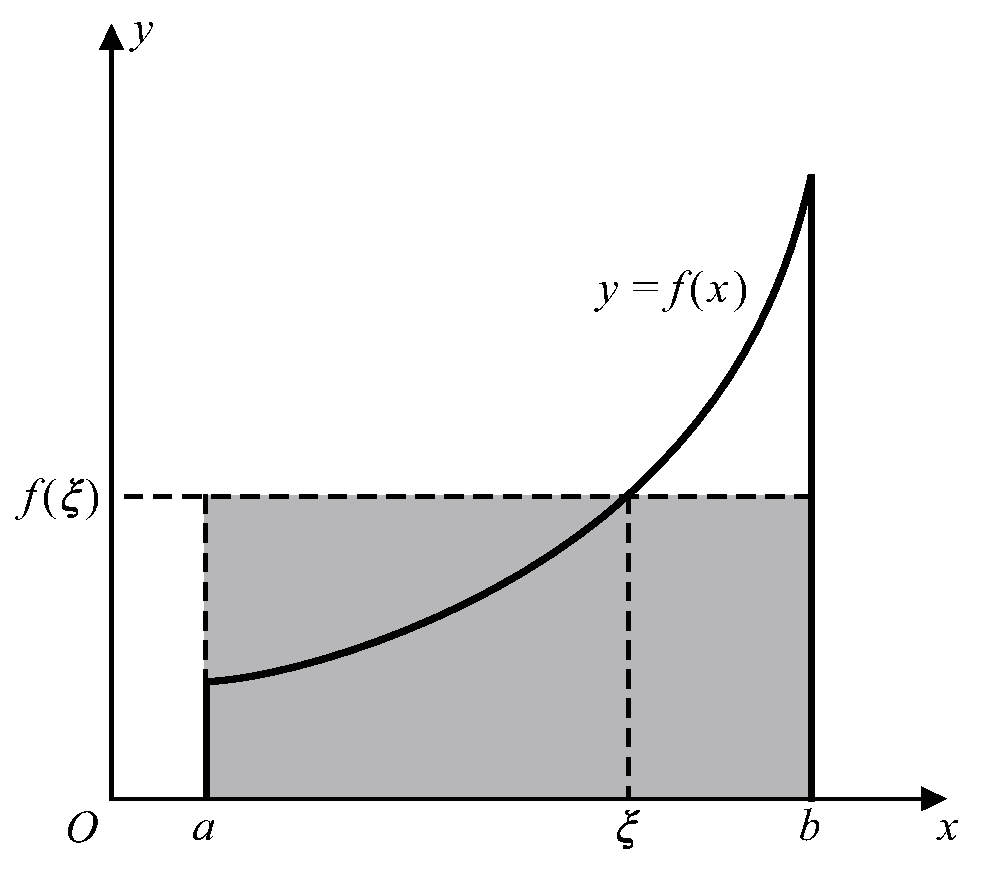
\includegraphics[width=0.7\linewidth]{pic/C-4/积分中值定理几何意义}
	\vspace*{-1em}
	\captionof{figure}{积分中值定理几何意义}
	\label{积分中值定理几何意义}
\end{minipage}

\subsection{变上限定积分函数的性质}
\noindent 1.\enspace 变上限定积分函数的定义\\
\hspace*{2em} 设函数$f(x)$在区间$[a,b]$上连续,并且设$x$为$[a,b]$上的一点,那么我们称函数
\begin{equation}
	F(x)=\int_{a}^{x}f(x) \,\d x
\end{equation}
为\highlight{dy}{\index{BSXJFHS@变上限定积分函数}变上限定积分函数}。由于定积分的值与标记变量无关,为了避免混淆,我们通常记作
\begin{equation}
	F(x)=\int_{a}^{x}f(t)\,\d t
\end{equation}
2.\enspace 变上限定积分函数的重要性质

\theorem[变上限定积分函数的性质]
设函数$f(x)$在区间$[a,b]$上连续,那么变上限定积分函数
\begin{equation}
	\nonumber
	F(x)=\int_{a}^{x}f(t) \,\d t
\end{equation}
在区间$[a,b]$上可导,且导函数为
\begin{equation}
	\nonumber
	F‘(x)=\frac{\d}{\d x}\int_{a}^{x}f(t) \,\d t=\d x  \hspace{1em}(a\leq x\leq b)
\end{equation}
\proof 由积分中值定理,对于任意$x,x+\Delta x\in[a,b]$,都至少存在一点$\xi\in[x,x+\Delta x]$,使得\vspace*{-1em}
\begin{equation}
	\nonumber
	F(x+\Delta x)-F(x)=\int_{a}^{x+\Delta x}f(t)\,\d t-\int_{a}^{x}f(t)\,\d t=\int_{a}^{x}f(t)\,\d t+\int_{x}^{x+\Delta x}f(t)\,\d t-\int_{a}^{x}f(t)\,\d t=\int_{x}^{x+\Delta x}f(t)\,\d t
\end{equation}
\begin{equation}
	\nonumber
	F(x+\Delta x)-F(x)=\int_{x}^{x+\Delta x}f(t)\d t=f(\xi)\Delta x
\end{equation}
即
\begin{equation}
	\nonumber
	\frac{F(x+\Delta x)-F(x)}{\Delta x}=f(\xi)
\end{equation}
由于任意$x,x+\Delta x\in[a,b]$上式都成立,那么我们不妨取$\Delta x\to 0$,即
\begin{equation}
	\nonumber
	\lim\limits_{\Delta x\to 0}	\frac{F(x+\Delta x)-F(x)}{\Delta x}=	\lim\limits_{\Delta x \to 0}f(\xi)
	\end{equation}
而
\begin{equation}
	\nonumber
	\lim\limits_{\Delta x\to 0}	\frac{F(x+\Delta x)-F(x)}{\Delta x}=F‘(x)
\end{equation}
又由于$\xi\in[x,x+\Delta x]$,$\Delta x\to0$,$\xi\to x$,故
\begin{equation}
	\nonumber
	\lim\limits_{\Delta x\to 0}f(\xi)=f(x)
\end{equation}
那么在区间$[a,b]$上有$F'(x)=f(x)$,考虑左端点和右端点的导数的情形,只需把上述推导过程中的$x$变成$a$即可。
故在区间$[a,b]$上都满足$F‘(x)=f(x)$
\\
这个定理说明了:\textbf{连续函数的变上限的积分就是该连续函数的一个原函数},即如果函数$f(x)$在$[a,b]$上连续,那么函数
\begin{equation}
	\nonumber
F(x)=\int_{a}^{x}f(t) \,\d t
\end{equation}
就是函数$f(x)$在$[a,b]$上的一个原函数。
\subsection{牛顿(Newton)—莱布尼茨(Leibniz)公式}

\theorem[微积分基本定理]
\label{theorem:4.8}
如果函数$F(x)$是连续函数$f(x)$在区间$[a,b]$上的一个原函数,那么
\begin{equation}
	\int_{a}^{b}f(t)\,\d t=F(b)-F(a)
\end{equation}
\proof 由\ref{theorem:4}$\,$知,$f(x)$的一个原函数为$\di F_0(x)=\int_{a}^{x}f(t)\,\d t$,那么$F'(x)-F'_0(x)=0$,故$F(x)-F_0(x)=C$($C$为常数)。又$f(x)$在区间$[a,b]$上连续,所以$F(x)-F_0(x)=C(C\text{为常数})$在区间$[a,b]$上恒成立。\\[0.5em]
\hspace*{2em} 不妨取$x=a$,由定积分的补充定义上下限相同时积分为0,那么$F(a)-F_0(a)=F(a)-0=C\Rightarrow C=F(a)$.\\[0.5em]
不妨取$x=b$,$\di F(b)-F_0(b)=F(b)-\int_{a}^{b}f(t)\,\d t=F(a) \Rightarrow \int_{a}^{b}=F(b)-F(a)$.
\vspace*{0.5em}

这个定理给了我们求定积分一种重要且简单的方法:找到被积函数的原函数,再计算两个端点函数值之差即可。

\vspace*{1.5em}

\noindent
\begin{minipage}{0.5\linewidth}
\section{定积分的应用}
	\subsection{曲线弧长的计算}
\hspace*{2em} 如图 \ref{弧长} 所示,设平面上给定的一条曲线弧$\wideparen{AB}$,其参数方程为:
\begin{equation}
	\begin{cases}
		\, x=x(t)\\
		 \, y=y(t)&
	\end{cases}
\end{equation}
\hspace*{2em} 当$t=a$时对应端点$A$,$t=b$时对应端点$B$。如果函数$x(t),y(t)$有连续的导函数$x'(t),y'(t)$那么这个曲线称为光滑曲线,光滑曲线总是可以计算弧长的。
\end{minipage}
\begin{minipage}{0.5\linewidth}
	\centering
	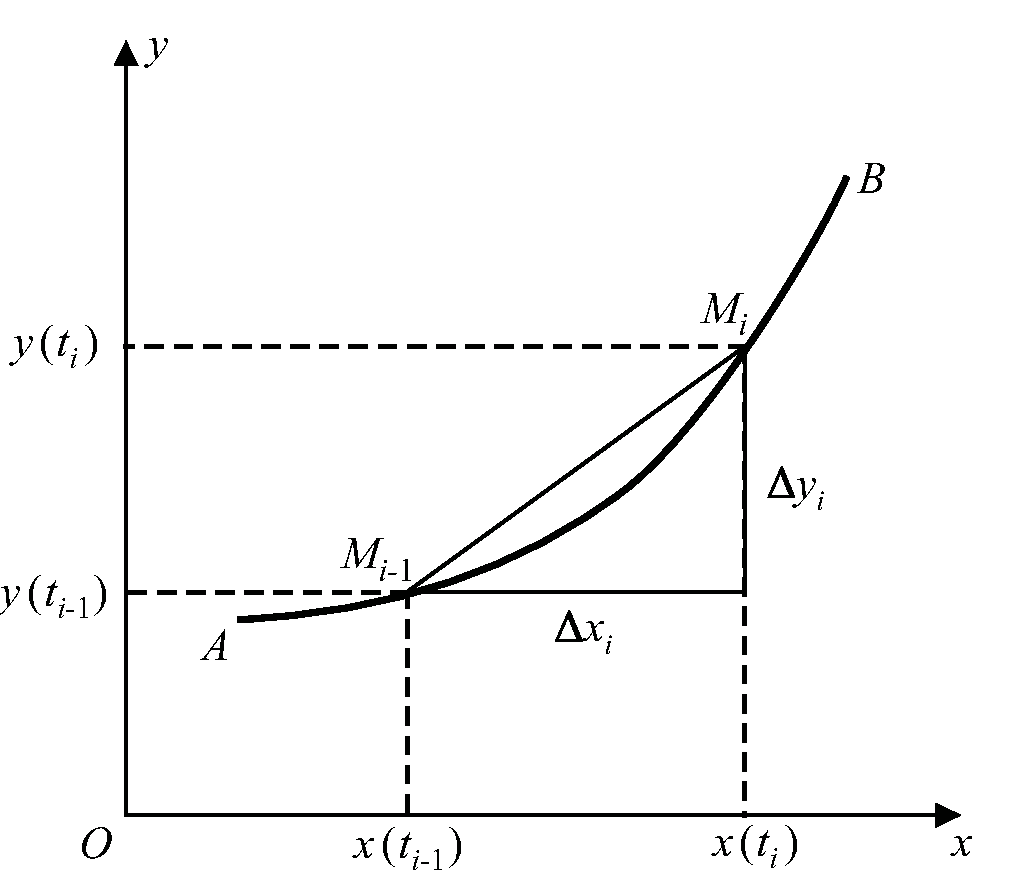
\includegraphics[width = 0.8\linewidth]{pic/C-4/弧长}
	\vspace*{-1em}
	\captionof{figure}{曲线弧长的计算}
	\label{弧长}
\end{minipage}

\par 我们将区间$[a,b]$分成$n$份:
\begin{equation}
	\nonumber
	a=t_0<t_1<\cdots<t_n=b
\end{equation}
那么在曲线弧$\wideparen{AB}$上也有相应的点;$M(x(t_i),y(t_i))$,i=0,1,$\cdots$,n.记
\begin{equation}l
	\Delta s_i=\wideparen{M_{i-1}M_i}\approx\overline{M_{i-1}M_i} =\sqrt{[x(t_i)-x(t_{i-1})]^2+[y(t_i)-y(t_{i-1})]^2}
\end{equation}
当区间无限小时,由导数定义:
\begin{equation}
	x'(t_{i-1})=\frac{x(t_i)-x(t_{i-1})}{t_i-t_{i-1}}\hspace{3em} y'(t_{i-1})=\frac{y(t_i)-y(t_{i-1})}{t_i-t_{i-1}}
\end{equation}
即
\begin{equation}
	x(t_i)-x(t_{i-1})=(t_i-t_{i-1})x^{'(t_{i-1})} \hspace*{3em}	y(t_i)-y(t_{i-1})=(t_i-t_{i-1})y^{'(t_{i-1})}
\end{equation}
故
\begin{align*}
	\Delta s_i=\wideparen{M_{i-1}M_i} &\approx \sqrt{[x(t_i)-x(t_{i-1})]^2+[y(t_i)-y(t_{i-1})]^2}=(t_i-t_{i-1})\sqrt{[x'(t_{i-1})]^2+[y'(t_{i-1})]^2}\\[0.5em]
	& =\sqrt{[x'(t_{i-1})]^2+[y'(t_{i-1})]^2}\Delta t_i
\end{align*}
其中$\Delta t_i=t_i-t_{i-1}$.令$\lambda=\max{\Delta t_i,1\leq i\leq n}\to0$,那么结合定积分的定义,此时每个区间长度都为无限小,那么
\begin{equation}
	C=\sum_{i=1}^{n}\Delta s_i=\lim\limits_{\lambda\to 0}\sum_{i=1}^{n}\sqrt{[x'(t_{i-1})]^2+[y'(t_{i-1})]^2}\Delta t_i=\int_{a}^{b}\sqrt{[x'(t)]^2+[y'(t)]^2}\,\d t
\end{equation}
所以,我们有下列曲线弧长的计算公式:
\\ 1.$\,$参数方程所确定的函数
\begin{equation}
	\int_{a}^{b}\sqrt{[x'(t)]^2+[y'(t)]^2}\,\d t
\end{equation}
2.一般函数(即令$x(t)=x,y(t)=f(x)$)
\begin{equation}
	\int_{a}^{b}\sqrt{1+[f'(t)]^2}\,\d t
\end{equation}
3.极坐标确定的函数$r=r(\theta)$,则$x(\theta)=r(\theta)\cos \theta,y(\theta)=r(\theta)\sin\theta$,
\begin{equation}
	\nonumber
	x'(\theta)=r'(\theta)\cos \theta-r(\theta)\sin \theta \hspace{2em} y'(\theta)=r'(\theta)\sin \theta+r(\theta)\cos \theta
\end{equation}
\begin{equation}
	\int_{a}^{b}\sqrt{[x'(\theta)]^2+[y'(\theta)]^2}\,\d \theta=\int_{a}^{b}\sqrt{[r'(\theta)]^2+[r(\theta)]^2}\,\d \theta
\end{equation}
\subsection{弧微分公式}
在前面我们已经知道弧长的计算公式,设弧长为$s(t)$,则
\begin{equation}
	s(t)=\int_{a}^{b}\sqrt{[x'(t)]^2+[y'(t)]^2}\,\d t
\end{equation}
对上式两边同时对$t$求导,得
\begin{equation}
	s'(t)=\sqrt{[x'(t)]^2+[y'(t)]^2}\hspace*{2em} \Rightarrow \hspace{2em} [s'(t)]^2=[x'(t)]^2+[y'(t)]^2 \hspace*{2em} \Rightarrow  \hspace*{2em} [\d s]^2=[\d x]^2+[\d y]^2
\end{equation}
我们便得到了弧微分公式:
\begin{equation}
	[\d s]^2=[\d x]^2+[\d y]^2
\end{equation}
\subsection{平面图形面积的计算}
\noindent 1.$\,$直角坐标情形
\par 有定积分定义可知,由曲线$y=f(x)(f(x)\geq 0)$及直线$x=a,x=b(a<b)$与$x$轴所围成的曲边梯形的面积$S$是
\begin{equation}
	S=\int_{a}^{b}f(x)\,\d x
\end{equation}
当求两个函数$f(x),g(x)$所围成部分的面积$S$时,一般有如下做法:

(1)$\,$找到函数$f(x),g(x)$的交点,并判断交点的区间内哪个函数大。

(2)$\,$求积分
\begin{equation}
	S=\int_{a}^{b}|f(x)-g(x)|\,\d x
\end{equation}
对于参数方程确定的函数,我们直接换元即可,即
\begin{equation}
	\nonumber
	\begin{cases}
		\, x=x(t)\\
		\, y=y(t)
	\end{cases}
\end{equation}
\begin{equation}
	S=\int_{a}^{b}y(t)\,\d [x(t)]=\int_{a}^{b}x'^{(t)}\cdot y(t)\,\d x
\end{equation}

\noindent
\begin{minipage}{0.7\linewidth}
	2.$\,$极坐标情形\\
\hspace*{2em} 如图 \ref{极坐标面积} 所示,设由曲线$\rho=\rho(\theta)$及射线$\theta=\alpha,\theta=\beta$围成一个图形(曲面扇形),且$\rho=\rho(\theta)$在$[\alpha.\beta]$上连续,$\rho(\theta)\geq0,0<\beta-\alpha\leq 2\pi$.\\
\hspace*{2em} 同样地,运用先分割求和再取极限的思想,将该区间分成$n$等份,对每个长度为无穷小的小区间,这个时候就可以用扇形面积的计算公式。因此,我们都可以计算抽根烟每个小区间的面积:
\begin{equation}
	S_i=\frac{1}{2}R^2\theta=\frac{1}{2}[\rho(\theta_i)]^2\Delta \theta
	\end{equation}
	然后进行求和:
\end{minipage}
\begin{minipage}{0.3\linewidth}
	\centering
	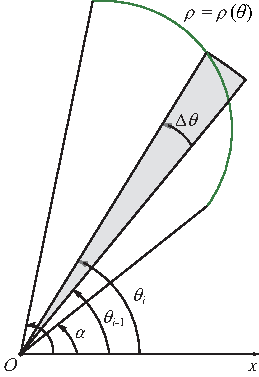
\includegraphics[width=0.7\linewidth]{pic/C-4/极坐标面积}
	\vspace*{-1.2em}
	\captionof{figure}{极坐标面积计算}
	\label{极坐标面积}
\end{minipage}

\begin{equation}
	S=\lim\limits_{n\to \infty}\sum_{i=1}^{n}S_i=\lim\limits_{n\to\infty}\sum_{i=1}^{n}\frac{1}{2}[\rho(\theta_i)]^2\Delta \theta=\frac{1}{2}\int_{\alpha}^{\beta}[\rho(\theta)]^2\,\d \theta_i
\end{equation}
这样我们便得到了极坐标面积公式:
\begin{equation}
	S=\frac{1}{2}\int_{\alpha}^{\beta}[\rho(\theta)]^2\,\d \theta
\end{equation}
\subsection{旋转体体积的计算}
综述:计算旋转体体积时,考虑图形的对称性有助于简化计算量,下面分几种常见的情况进行讲解。\\
\textbf{1.$\,$绕$x$轴旋转的情形}
\par 如图 \ref{x旋转} 所示,我们将区间$[a,b]$分成$n$份:
\begin{equation}
	\nonumber
	a=x_0<x_1<\cdots<x_n=b
\end{equation}
那么在曲面弧$\wideparen{AB}$上也即由相应的点:$M_i(x_i),f(x_i),i=0,1,\cdots,n$.\\
记$n$个小区间$[x_{i-1},x_i],i=0,1,\cdots,n$绕$x$轴所形成的旋转体的体积为$\Delta V_i$.\\
如果在每个小区间$[x_{i-1},x_i]$中取一点$\xi$,那么当$\Delta x_i\to0$时,每个小区间绕$x$轴所形成的旋转体都可以看成一个小圆柱,由圆柱的体积公式可得:
\begin{equation}
	\Delta V_i=\pi R^2 h=\lim\limits_{\Delta x_i\to0}\pi[f(\xi_i)]^2\Delta x_i
	\label{equ:1}
\end{equation}
\begin{figure}
	\centering
	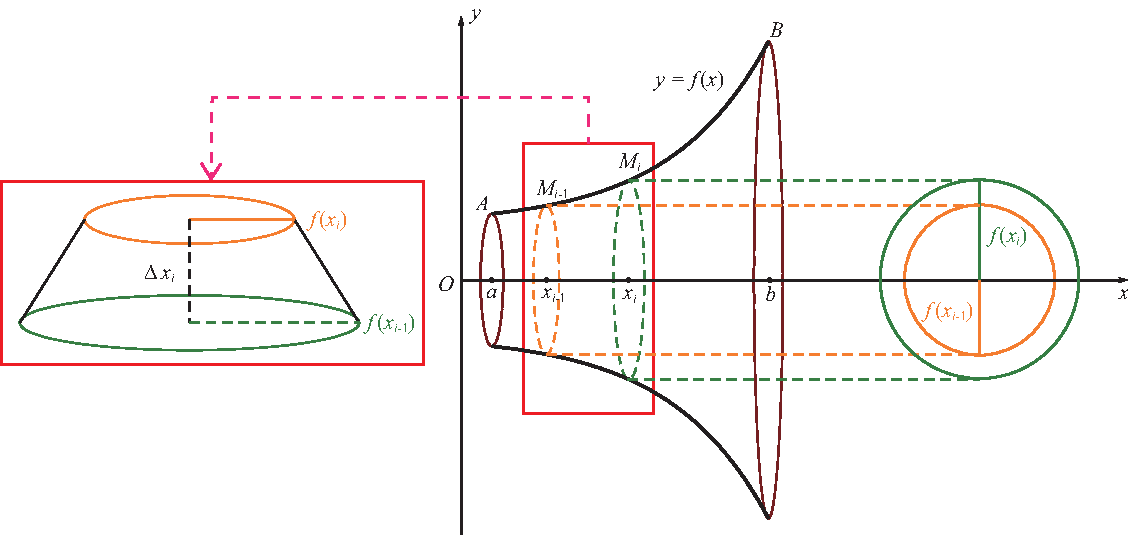
\includegraphics[width=0.9\linewidth]{pic/C-4/x旋转体积}
	\vspace*{-1em}
	\caption{绕$x$轴的旋转体体积的计算}
	\label{x旋转}
\end{figure}
由于$\Delta x_i\to0$,不妨取$\xi_i=x_i$,那么式\eqref{equ:1}可以写成
\begin{equation}
	\Delta V_i=\lim\limits_{\Delta x_i\to0}\pi[f(x_i)]^2\Delta x_i
\end{equation}
那么,
\begin{equation}
	V=\sum_{i=1}^{n}\Delta V_i=\lim\limits_{\Delta x_i\to0}\sum_{i=1}^{n}\pi[f(x_i)]^2\Delta x_i=\pi\int_{a}^{b}[f(x)]^2\,\d x
\end{equation}
即
\begin{equation}
	V=\pi\int_{a}^{b}[f(x)]^2\,\d x
\end{equation}

\noindent \textbf{2.$\,$绕$y$轴旋转的情形}
\par 绕$y$轴旋转的情形只需要将绕$x$轴旋转的情形中的函数$y=f(x)$改为$x=g(y)$即可,其中$g(y)$是$f(x)$的反函数,即
\begin{equation}
	V=\pi\int_{c}^{d}[g(y)]^2\,\d y
\end{equation}
其图像大致如图 \ref{y旋转} 所示。
\begin{figure}[!htb]
	\centering
	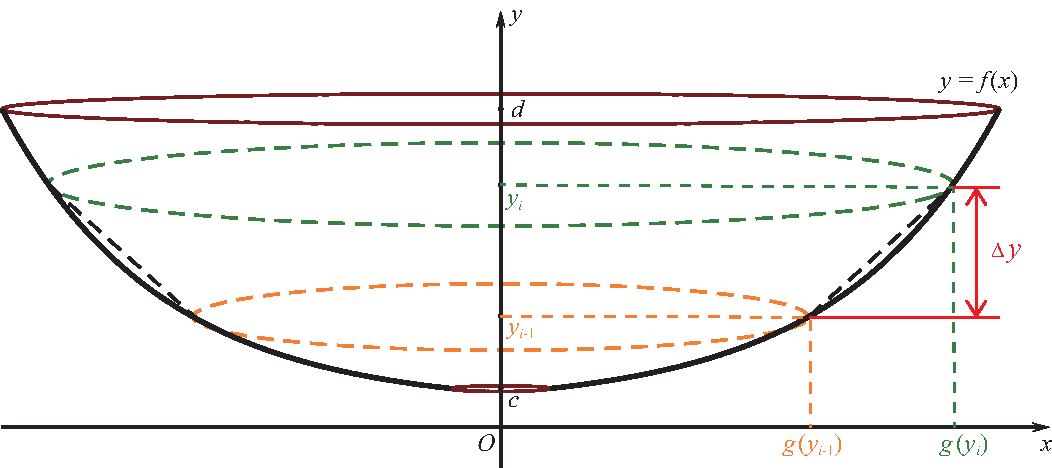
\includegraphics[width=0.7\linewidth]{pic/C-4/y旋转体积}
	\vspace*{-1em}
	\caption{绕$y$轴的旋转体体积的计算}
	\label{y旋转}
\end{figure}

\textbf{3.$\,$绕定直线旋转的情形}
\par 通常我们只需考虑绕直线$x=c$或直线$y=c$($c$为常数)的情况。
\subsection{旋转体侧面积的计算}
\par 设$A$为旋转体的侧面积,$s$为曲线的弧长,那么
\begin{equation}
	\d A=2\pi\, \d s
\end{equation}
若绕$x$轴旋转,那么得到的公式为
\begin{equation}
	 A=2\pi \int_{a}^{b}f(x)\,\d s=2\pi\int_{a}^{b}\sqrt{1+[f'(x)]^2}\,\d x
\end{equation}
若绕$y$轴旋转,那么得到的公式为
\begin{equation}
	A=2\pi \int_{c}^{d}g(x)\,\d s=2\pi\int_{c}^{d}\sqrt{1+[g'(y)]^2}\,\d y
\end{equation}





